\documentclass[11pt]{report}
\usepackage{geometry}                % See geometry.pdf to learn the layout options. There are lots.
\geometry{letterpaper}                   % ... or a4paper or a5paper or ... 
%\geometry{landscape}                % Activate for for rotated page geometry
%\usepackage[parfill]{parskip}    % Activate to begin paragraphs with an empty line rather than an indent
\usepackage{graphicx}
\usepackage{amssymb}
\usepackage{epstopdf}
\DeclareGraphicsRule{.tif}{png}{.png}{`convert #1 `dirname #1`/`basename #1 .tif`.png}

\title{AIS Storage user guide}
\author{Xavier Tordoir}
%\date{}                                           % Activate to display a given date or no date

\begin{document}
\maketitle
\tableofcontents
\part{Prerequisites}
\chapter{Introduction}
The AIS storage system is a cloud based storage system. As such, storage operations are performed by HTTP requests exclusively, either through the web application or the REST API. The system is very similar to the Amazon S3 or Google Storage products. The main features differentiating these products from our solution is that the physical storage is provided by third parties and not exclusively by us.
\section{Definitions and concepts}
\subsection{bucket}
A Bucket is a container for files and objects. The user can consider a bucket as a kind of virtual disk. This means that buckets cannot be nested, they are always the root of a set of data to be organized within the bucket. Sharing data with collaborators and customers is configured at the bucket level. The user can so consider a bucket as a workspace or project allowing to grant access on its content to other selected users.
\subsection{bucket metadata}
Bucket Metadata are sets of key-value pairs associated with a bucket. These metadata allow the owner of a bucket to configure the behaviour of the bucket with respect to data storage (see �...), and to add some general information about the bucket.
\subsection{object}
Objects are the elements contained in a bucket, no object exists outside of a bucket.  All objects have a \emph{key} with is a text uniquely identifying the object within the bucket. In a simple usage scenario, the \emph{key} is the path of a file or directory within the bucket.\\
An object is actually a pointer to a unit of data. This object can point to a file, a directory or any other type of data that can be stored in the form of object metadata. 
\subsection{object metadata}
Metadata in the form of key-value pairs can be associated with objects. This mechanism is used for example to identify an object as a file on a physical storage device. These metadata allow to configure the behaviour of an object (for example a file can be downloaded), or for the user to add some general information about the object.
\subsection{store}
While the list of objects stored in buckets as well as metadata are maintained in a database, files are stored on physical disks. The system is able to access these physical files through the concept of stores. A store is an ssh connection to a server providing storage space. This connection is a username, a server address (IP or dns) and a root directory under which all data are stored.
\part{User guide: web interface}
\chapter{Store management}
The use of the storage system relies on a database used to store the bucket and objects definitions and metadata and on a number of \emph{store} to store the files. The database is provided by the AIS storage middleware, while the stores are dynamically plugged on the system and access is granted to users. So store management is the basics to be able to manage files in the system.
\section{Store creation}
The creation of a \emph{store} is reserved to users with the role allowing them to manage stores. This role can be requested on the account tab on the web application.
\begin{figure}[htbp]
   \centering
   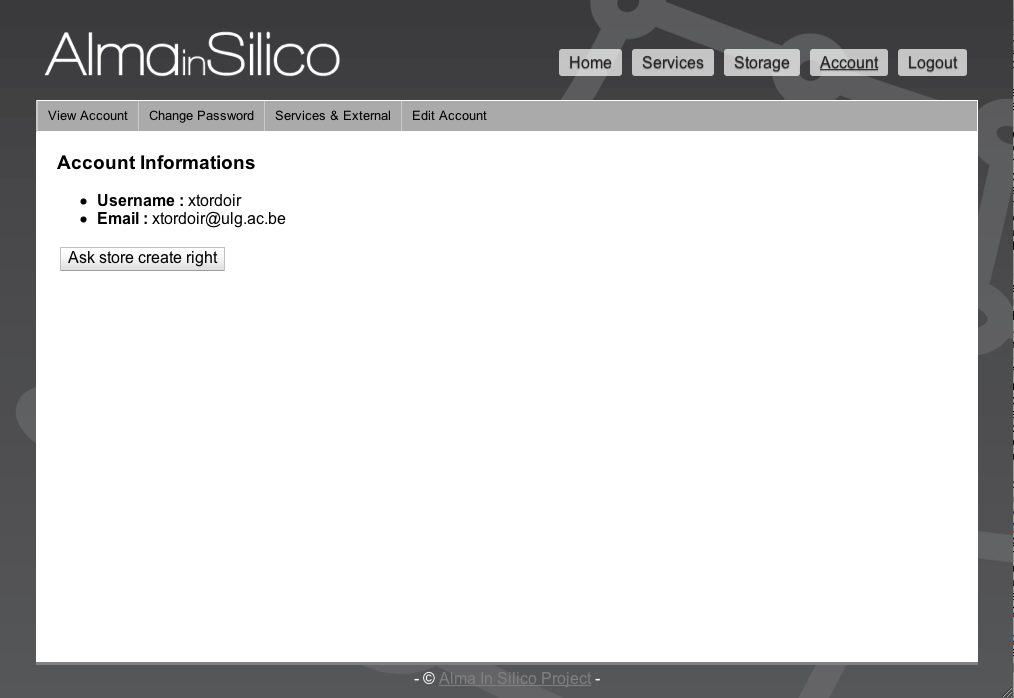
\includegraphics[width=1.0\linewidth]{askstorec.png} % requires the graphicx package
   \caption{Request store creation rights}
   \label{fig:example}
\end{figure}
With this right, a store can be created.
\subsection{Store definition}
The minimal information required to create a store consists in the following fields:
\begin{itemize}
\item namespace: a unique string identifier for the store, 8 characters maximum, alphanumeric
\item username: the username to be used to login on the remote server
\item store\_url: the server IP or dns
\item path: the absolute path on the server where all data will be stored.
\item tmp: the absolute path on the server where some temporary data can be stored during local copy processes (see ...)
\item \_default: a boolean tag setting the default store
\item description: the text description of the store
\end{itemize}
Store creation is done exclusively on the web application, in the storage tab under the store panel:
\begin{figure}[htbp]
   \centering
   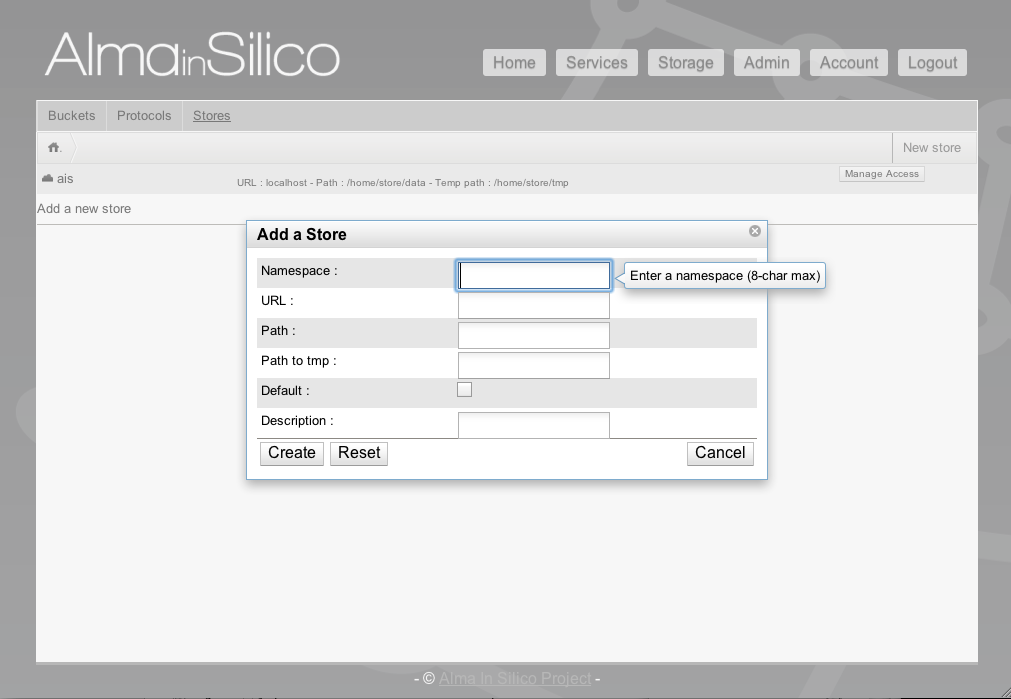
\includegraphics[width=1.0\linewidth]{createstore.png} % requires the graphicx package
   \caption{Store creation form}
   \label{fig:example}
\end{figure}
\subsection{TODO: public key download and installation - store validation}
\section{store rights management}
A store administrator (its creator just after creation) is able to grant rights on the store. The global rights are:
\begin{itemize}
\item visibility: control whether the store is visible to all users. If yes, all users in the system are aware that the store exists, although they don't have access to the store, they are able to make a request to access it. The store administrator will accept or reject such requests.
\item writable for all: this controls whether all users have a write access on the store. This only works if the store is visible.
\end{itemize}
The rights granted to users (by email address) are:
\begin{itemize}
\item Admin: read and write access, administration rights (users management)
\item Users: read and write access, can download and upload files on the store
\item viewer: read access, can download files from the store
\end{itemize}
\begin{figure}[htbp]
   \centering
   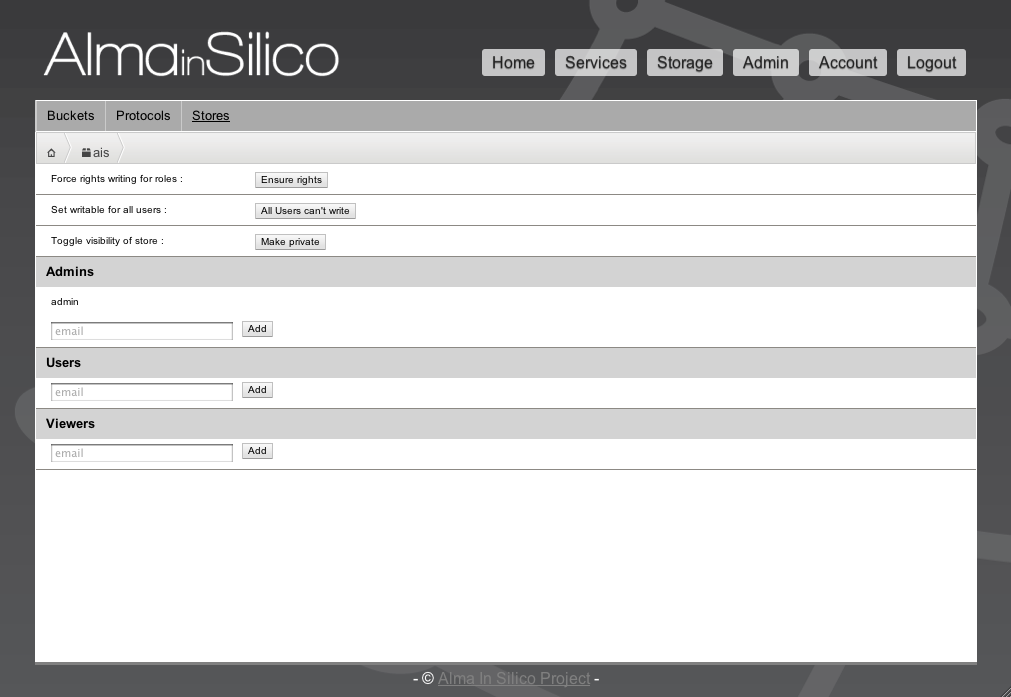
\includegraphics[width=1.0\linewidth]{storeacl.png} % requires the graphicx package
   \caption{Store rights management page}
   \label{fig:example}
\end{figure}
\section{Store API}

\begin{verbatim}
NO STORE API AVAILABLE
\end{verbatim}
% BUCKET MANAGEMENT
\chapter{Bucket management}
\section{Bucket creation}
\subsection{Bucket definition}
In order to create a bucket, the minimal information required are the following mandatory attributes:
\begin{itemize}
\item name: the name of the bucket, unique across all users buckets
\item description: a text description of the bucket
\end{itemize}
\subsection{Bucket metadata}
A bucket can be created with a number of options. These options will influence the way data files are physically stored and are set as bucket metadata:
\begin{itemize}
\item store.multiplicity: the multiplicity of stores used by the bucket, can be \emph{unique} or \emph{multiple}. A multiple store allows to store files on multiple devices, it is the default value.
\item store.default: the default store, this option is mandatory if store.multiplicity is \emph{unique}.
\item fs.mapping: the filesystem mapping type, can be either \emph{mirror} or \emph{tree}. The mirror mapping means that object keys are paths on the physical storage. The default is \emph{mirror} as it allows to manage data as in a filesystem. In a \emph{mirror} configuration it is not possible for a node that is not a leaf to point to a file.
\end{itemize}
These options cannot be changed once the bucket is created.\\
Other user defined metadata are managed by the user and remain dynamic after the bucket creation.
\section{Bucket rights management}

\section{Bucket API}

\chapter{Object management}
\section{Object creation}
\subsection{Object definition}
\subsection{Object as File}
\subsection{Object metadata}
\section{Object API}
\part{User guide: REST API}
\chapter{Store}
\emph{Stores} cannot be managed with the API, only the web interface allows to create and manage access control on stores.
\chapter{Bucket} 
\section{Bucket creation}
\section{Bucket }
\subsection{Object as File}
\subsection{Object metadata}
\section{Object API}


\end{document}  